\section{Evaluation}

We evaluate the framework on a Home Assistant prototype. The evaluation focuses on detection effectiveness and the execution time of the static and runtime components.

\subsection{Experiment Setup}

\begin{figure}[htbp]
	\centering
	
\includegraphics[width=0.9\textwidth]{figure/smarthome.png}
	\caption{Smart Home Floor Plan used for Evaluation}
	\label{smarthome_floorplan}
\end{figure}

The testbed is implemented in Home Assistant, which stores automation rules in YAML files and therefore provides a convenient source for extracting TCAE models. It is built from the floor plan in Figure~\ref{smarthome_floorplan} and contains seven functional zones and 32 smart devices. Physical-channel analysis involves six sensor-equipped zones.

Spatial connectivity determines whether environmental effects can propagate across zones. For example, the Porch and the Living Room are connected, whereas the Bedroom is physically isolated from them.

% \begin{table}[htbp]
% 	\caption{Physical Channel Configuration Used in Evaluation}
% 	\label{physical_channel}
% 	\centering
% 	\begin{adjustbox}{width=\textwidth}
% 	\begin{tabular}{l|l|l}
% 		\hline
% 		\textbf{Zone} & \textbf{Channel} & \textbf{Trend} \\
% 		\hline
% 		Outdoor & Brightness & Increase/Decrease \\
% 		\hline
% 		Porch & Brightness & Increase/Decrease \\
% 		\hline
% 		Kitchen & Brightness, Temperature & Increase/Decrease \\
% 		\hline
% 		Living Room & Brightness, Humidity, Temperature & Increase/Decrease \\
% 		\hline
% 		Bedroom & Brightness, Temperature & Increase/Decrease \\
% 		\hline
% 		Greenhouse & Brightness, Temperature & Increase/Decrease \\
% 		\hline
% 	\end{tabular}
% 	\end{adjustbox}
% \end{table}

Table~\ref{Testbeds} summarizes the 17 automation rules deployed in the testbed. For the Entity Safety Configuration, we define preferred safe states for four safety-sensitive entities: the Water Valve \circled{18} is preferred to remain ``open'' to preserve fire supply, the Sprinkler \circled{20} is preferred to remain ``enabled'', the Bedroom Window \circled{26} is preferred to remain ``closed'', and the Smart Door Lock \circled{3} is preferred to remain ``locked''.

\begin{table*}[htbp]
	\caption{Experimental Smart Home Automation Rules (R1--R17) in compact TCA form.}
	\label{Testbeds}
	\centering
	\small
	\begin{adjustbox}{width=\textwidth}
	\begin{tabular}{c|p{3.2cm}|p{1.8cm}|p{4.0cm}|c|l}
		\hline
		\textbf{Rule ID} & \textbf{Trigger} & \textbf{Condition} & \textbf{Action} & \textbf{Zone} & \textbf{Devices} \\
		\hline
		R1  & DL1 = unlocked & B1 $< 50$\,lux & L1 = on, L2 = on & Outdoor & \circled{1} \circled{2} \circled{3} \circled{4} \\
		\hline
		R2  & L6 = off & -- & DL1 = unlocked & Porch & \circled{3} \circled{30} \\
		\hline
		R3  & M1 = detected & B2 $< 50$\,lux & L2 = on & Porch & \circled{4} \circled{5} \circled{6} \\
		\hline
		R4  & M2 = detected & B3 $< 50$\,lux & L3 = on & Living Room & \circled{7} \circled{8} \circled{10} \\
		\hline
		R5  & HT1.humidity $< 40\%$ & HU1 = off & HU1 = on & Living Room & \circled{9} \circled{11} \\
		\hline
		R6  & HT1.humidity $> 60\%$ & -- & HU1 = off & Living Room & \circled{9} \circled{11} \\
		\hline
		R7  & HT1.temperature $< 24$\celsius & -- & UFH1 = on & Living Room & \circled{9} \circled{12} \\
		\hline
		R8  & HT1.temperature $> 30$\celsius & -- & AC1 = on, setpoint = $27$\celsius & Living Room & \circled{9} \circled{13} \\
		\hline
		R9  & M3 = detected & B4 $< 50$\,lux & L4 = on & Kitchen & \circled{14} \circled{15} \circled{17} \\
		\hline
		R10 & WLS1 = detected & -- & WV1 = closed & Kitchen & \circled{16} \circled{18} \\
		\hline
		R11 & SD1 = triggered & -- & SP1 = enabled & Kitchen & \circled{19} \circled{20} \\
		\hline
		R12 & M4 = detected & B5 $< 50$\,lux & L5 = on & Bedroom & \circled{21} \circled{22} \circled{24} \\
		\hline
		R13 & time = 7 PM & -- & HTR1 = on & Bedroom & \circled{25} \\
		\hline
		R14 & T1 $\ge 30$\celsius & -- & W1 = open, HTR1 = off & Bedroom & \circled{23} \circled{25} \circled{26} \\
		\hline
		R15 & DL1 = locked & -- & L2 = off, L6 = off & Outdoor & \circled{3} \circled{4} \circled{30} \\
		\hline
		R16 & time = 7 PM & -- & HTR2 = on & Greenhouse & \circled{31} \\
		\hline
		R17 & T2 $\ge 32$\celsius & -- & SK1 = open, HTR2 = off & Greenhouse & \circled{29} \circled{31} \circled{32} \\
		\hline
	\end{tabular}
	\end{adjustbox}
\end{table*}

\subsection{Effectiveness of Conflict Detection}

We manually inspected the 17 automation rules and established ground truth for interaction pairs and conflict cases under the configured Entity Safety Configuration. We then triggered the relevant rules in Home Assistant and compared our framework with IoTMediator. Static analysis identified 58 rule interactions in the testbed: 2 Trigger Interactions, 2 Condition Interactions, 10 Action Interactions, 7 Indirect Trigger Interactions, 15 Indirect Condition Interactions, and 22 Indirect Action Interactions. Applying the Entity Safety Configuration pruned the RIDG and retained only the interaction edges corresponding to candidate rule conflicts for runtime monitoring.

Representative cases illustrate the effect of this filtering. For R5-R6, the corresponding interaction edge is not retained because the pair forms a user-expected closed-loop humidity control and does not involve a safety-sensitive entity. In the direction $R10 \rightarrow R11$, the interaction edge is retained because closing the main water valve can deprive the enabled sprinkler of the water supply required for fire response; this case is recorded as an Indirect Action Conflict. In the reverse direction $R11 \rightarrow R10$, sprinkler activation may trigger the leak sensor and subsequently the valve-closing rule, so the edge is recorded as an Indirect Trigger Conflict. The pairs $R13 \rightarrow R14$ and $R16 \rightarrow R17$ have similar physical logic, but only the bedroom pair is retained because the bedroom window is safety-sensitive whereas the greenhouse skylight is not. In addition, the system retains the chain $R15 \rightarrow R2$ as a Trigger Conflict because locking the door may subsequently cause it to be unlocked through the greenhouse-light trigger.

Table~\ref{conflict_detection_result} reports selected conflict-related rule pairs, including all manually confirmed conflict cases under the configured Entity Safety Configuration and representative non-conflict pairs flagged by at least one system. One rule pair may satisfy multiple static conflict categories, so multiple categories may be reported for the same pair. For our framework, the table reports the six static conflict categories used during RIDG/RCDG construction. Compared with IoTMediator, our framework detected all manually confirmed conflict cases in this testbed. IoTMediator missed the interaction between R10 and R11 because it does not model the indirect physical effect between the valve and the sprinkler, and it incorrectly flagged the greenhouse pair R16-R17 because it lacks zone awareness. It also reported non-risky cases such as R3-R15. These results indicate that considering both physical relevance and application-scenario-specific safety boundaries helps reduce false positives while preserving the conflict cases confirmed in this testbed. As a qualitative highlight, an external audit with DeepSeek-R1 also suggested that the generated reports preserve sufficient causal and safety information for inspection.

\begin{table*}[htbp]
	\centering
	\caption{Selected conflict-related rule pairs and detection results. Columns include all manually confirmed conflict cases under the configured Entity Safety Configuration and representative non-conflict pairs flagged by at least one system. Here, $\checkmark$, $\times$, and -- denote true positives, false positives, and unreported pairs, respectively.}
	\label{conflict_detection_result}
	\resizebox{\textwidth}{!}{
		\begin{tabular}{|c|l|c|c|c|c|c|c|c|c|c|c|c|c|}
			\hline
			& \multicolumn{1}{c|}{\textbf{Classification}} & \textbf{R2-R1} & \textbf{R3-R15} & \textbf{R5-R6} & \textbf{R6-R5} & \textbf{R10-R11} & \textbf{R11-R10} & \textbf{R13-R14} & \textbf{R14-R13} & \textbf{R15-R2} & \textbf{R15-R3} & \textbf{R16-R17} & \textbf{R17-R16} \\ \hline

			\multirow{6}{*}{\textbf{Ours}}
			& Trigger Conflict             & -- & -- & -- & -- & -- & -- & -- & -- & $\checkmark$ & -- & -- & -- \\ \cline{2-14}
			& Condition Conflict           & -- & -- & -- & -- & -- & -- & -- & -- & -- & -- & -- & -- \\ \cline{2-14}
			& Action Conflict              & -- & -- & -- & -- & -- & -- & $\checkmark$ & $\checkmark$ & -- & -- & -- & -- \\ \cline{2-14}
			& Indirect Trigger Conflict    & -- & -- & -- & -- & -- & $\checkmark$ & $\checkmark$ & -- & -- & -- & -- & -- \\ \cline{2-14}
			& Indirect Condition Conflict  & -- & -- & -- & -- & -- & -- & -- & -- & -- & -- & -- & -- \\ \cline{2-14}
			& Indirect Action Conflict     & -- & -- & -- & -- & $\checkmark$ & $\checkmark$ & $\checkmark$ & $\checkmark$ & -- & -- & -- & -- \\ \hline

			\multirow{7}{*}{\textbf{IoTMediator}}
			& Condition Enabling/Disabling & -- & -- & $\times$ & $\times$ & -- & -- & -- & -- & -- & -- & -- & -- \\ \cline{2-14}
			& Race Condition               & -- & -- & -- & -- & -- & -- & -- & -- & -- & -- & -- & -- \\ \cline{2-14}
			& Potential Race Condition     & -- & $\times$ & $\times$ & $\times$ & -- & -- & $\checkmark$ & $\checkmark$ & -- & $\times$ & $\times$ & $\times$ \\ \cline{2-14}
			& Chained Execution            & $\times$ & -- & -- & -- & -- & -- & -- & -- & $\checkmark$ & -- & -- & -- \\ \cline{2-14}
			& Action Revert                & -- & -- & -- & -- & -- & -- & -- & -- & -- & -- & -- & -- \\ \cline{2-14}
			& Infinite Loop                & -- & -- & -- & -- & -- & -- & -- & -- & -- & -- & -- & -- \\ \cline{2-14}
			& Condition Bypass             & -- & -- & -- & -- & -- & -- & -- & -- & -- & -- & -- & -- \\ \hline
		\end{tabular}
	}
	\par\vspace{2pt}
	\footnotesize
\end{table*}

\subsection{Performance}

% \begin{figure}[htbp]
%   \centering
%   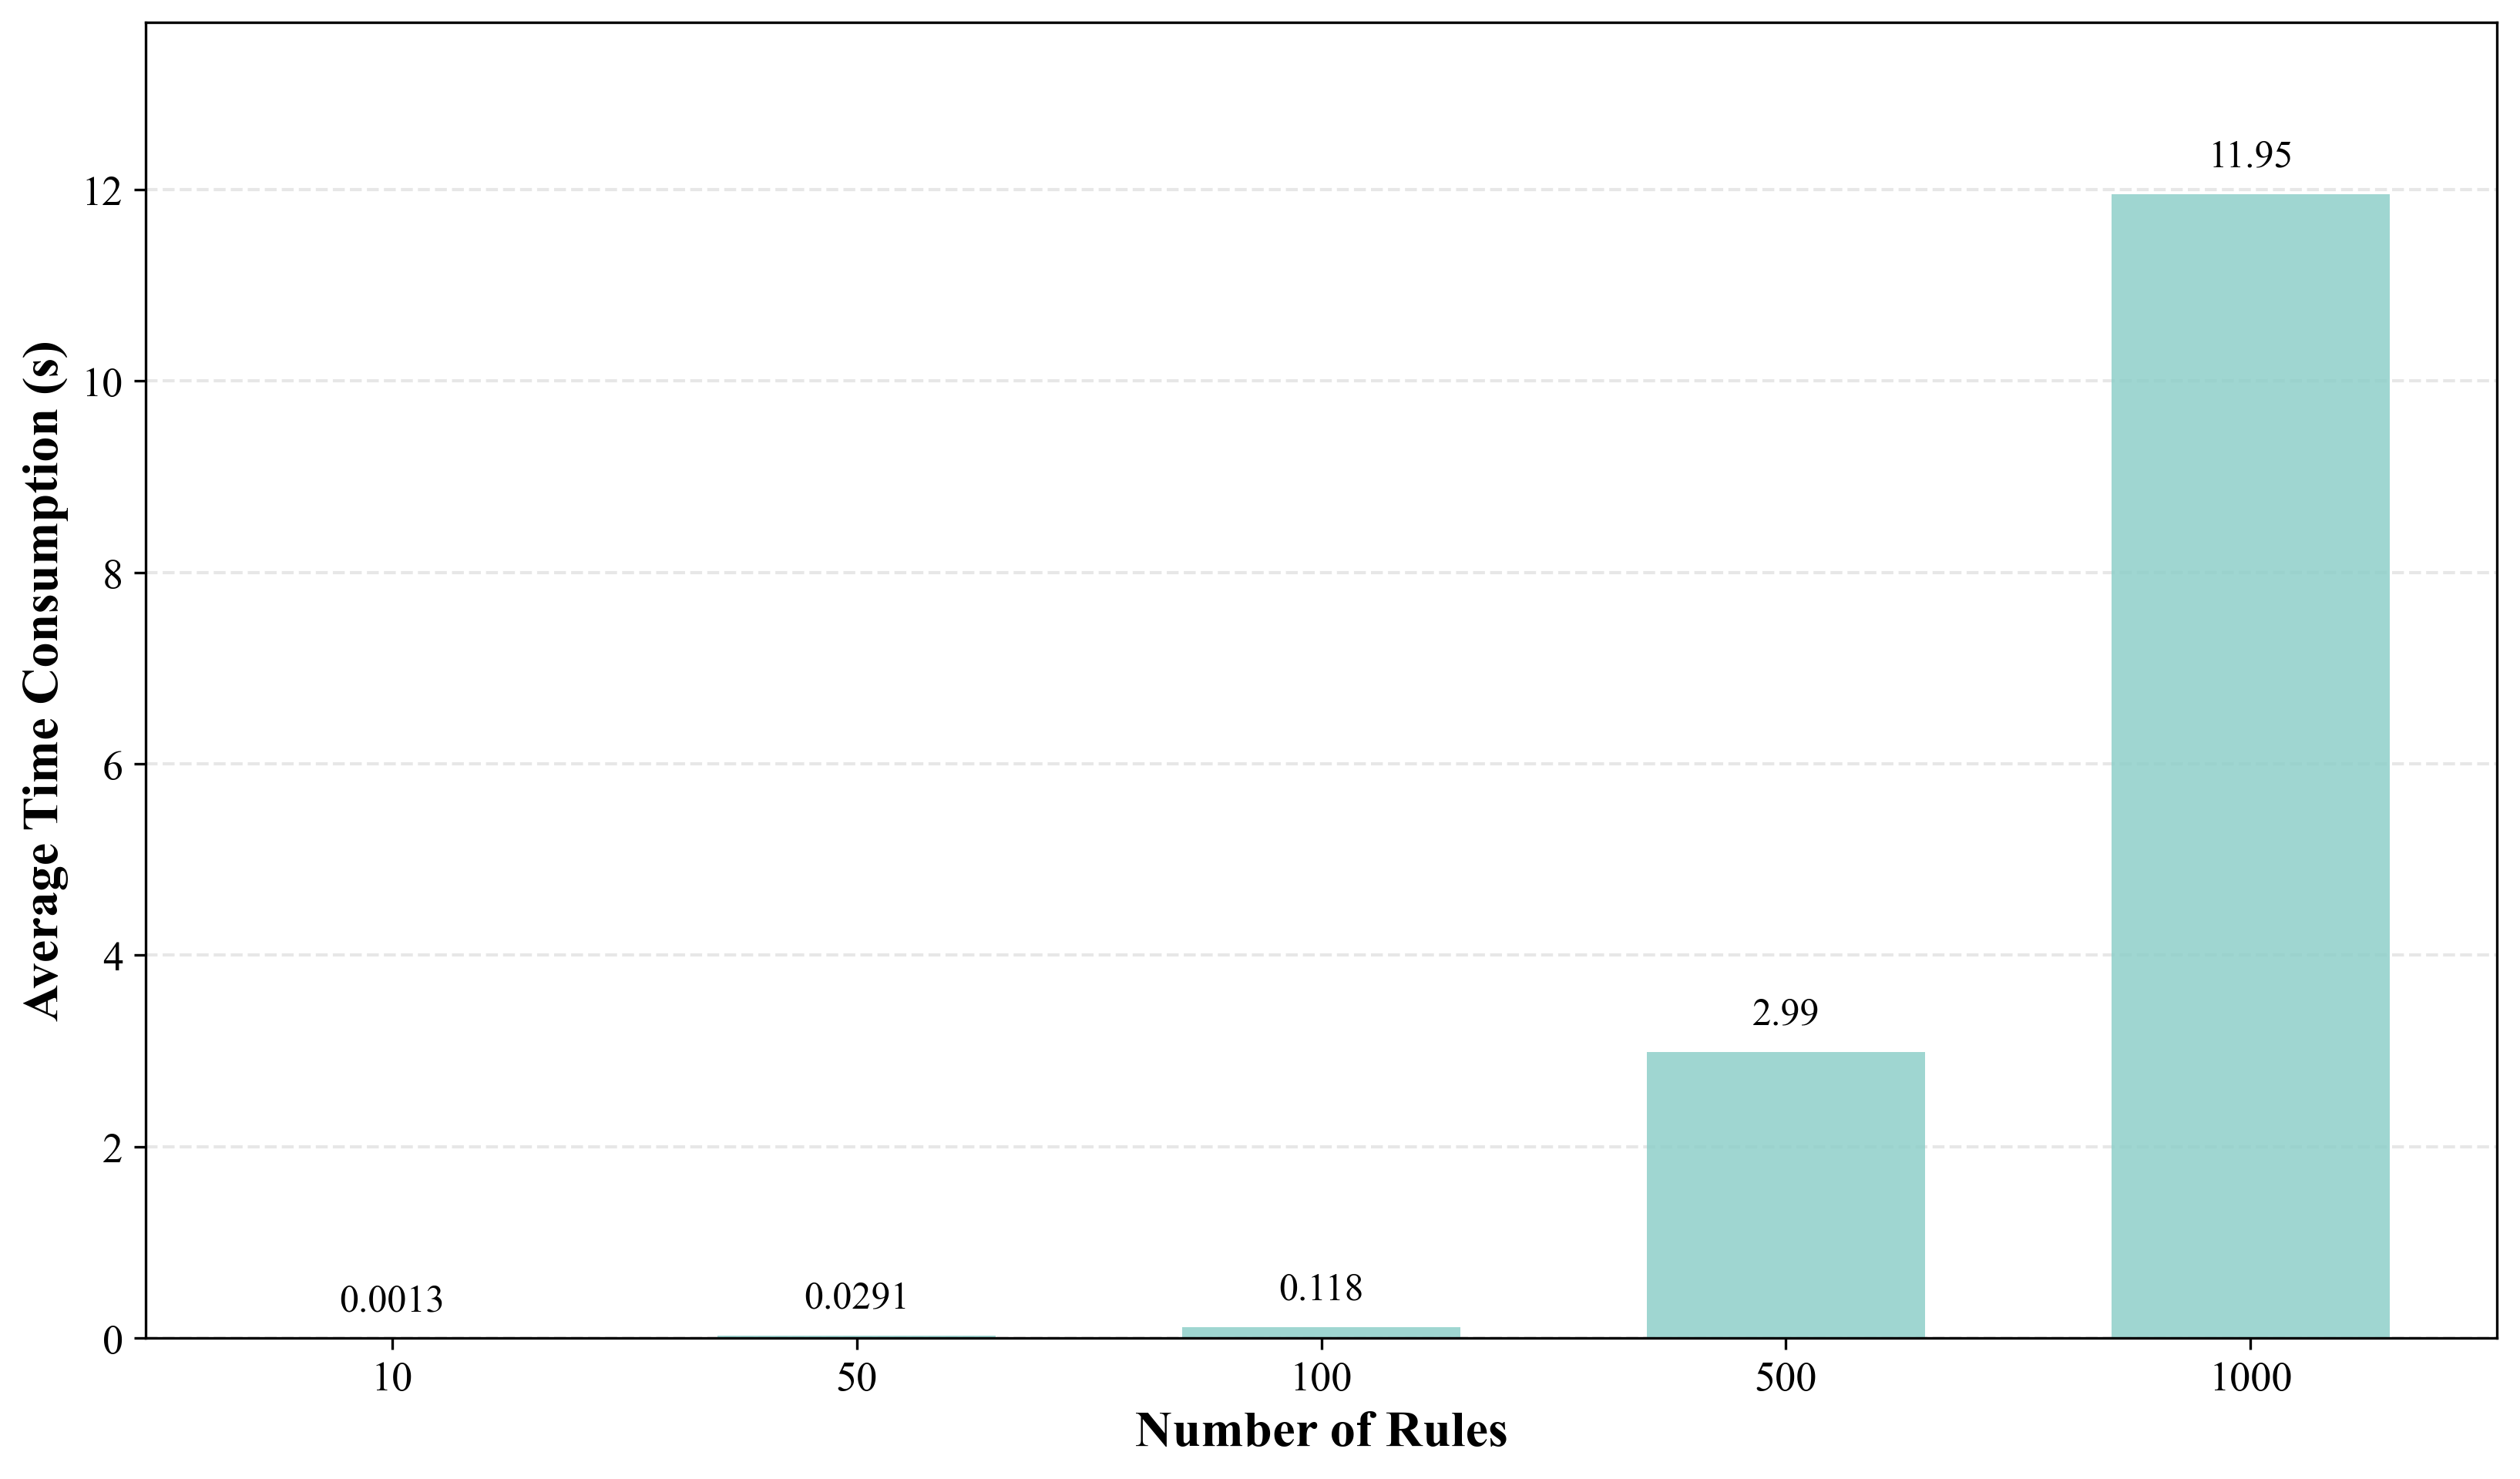
\includegraphics[width=0.8\textwidth]{figure/performance.png}
%   \caption{Static analysis execution time under different rule-set sizes.}
%   \label{performance_static_analysis}
% \end{figure}

\begin{figure*}[t]
  \centering
  \begin{minipage}[t]{0.48\linewidth}
        \begin{subfigure}{\linewidth}
            \centering
            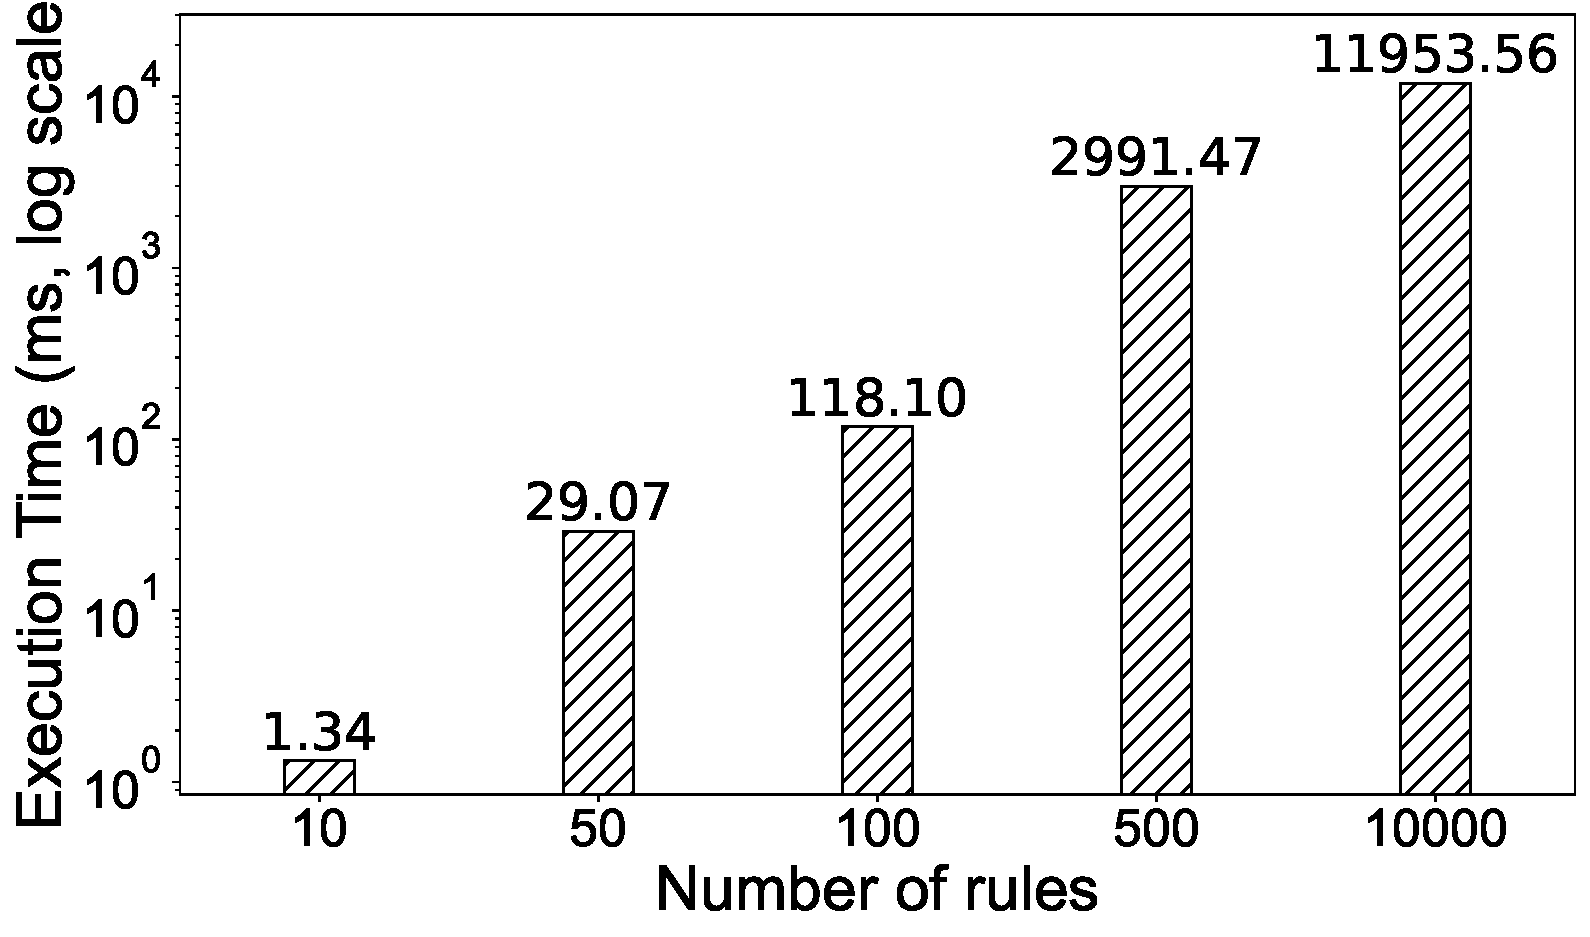
\includegraphics[width=\linewidth]{figure/static.pdf}
            \caption{Static analysis execution time under different rule-set sizes.}            
            \label{subfig:static}
        \end{subfigure}
  \end{minipage}
    \begin{minipage}[t]{0.48\linewidth}
        \begin{subfigure}{\linewidth}
            \centering
            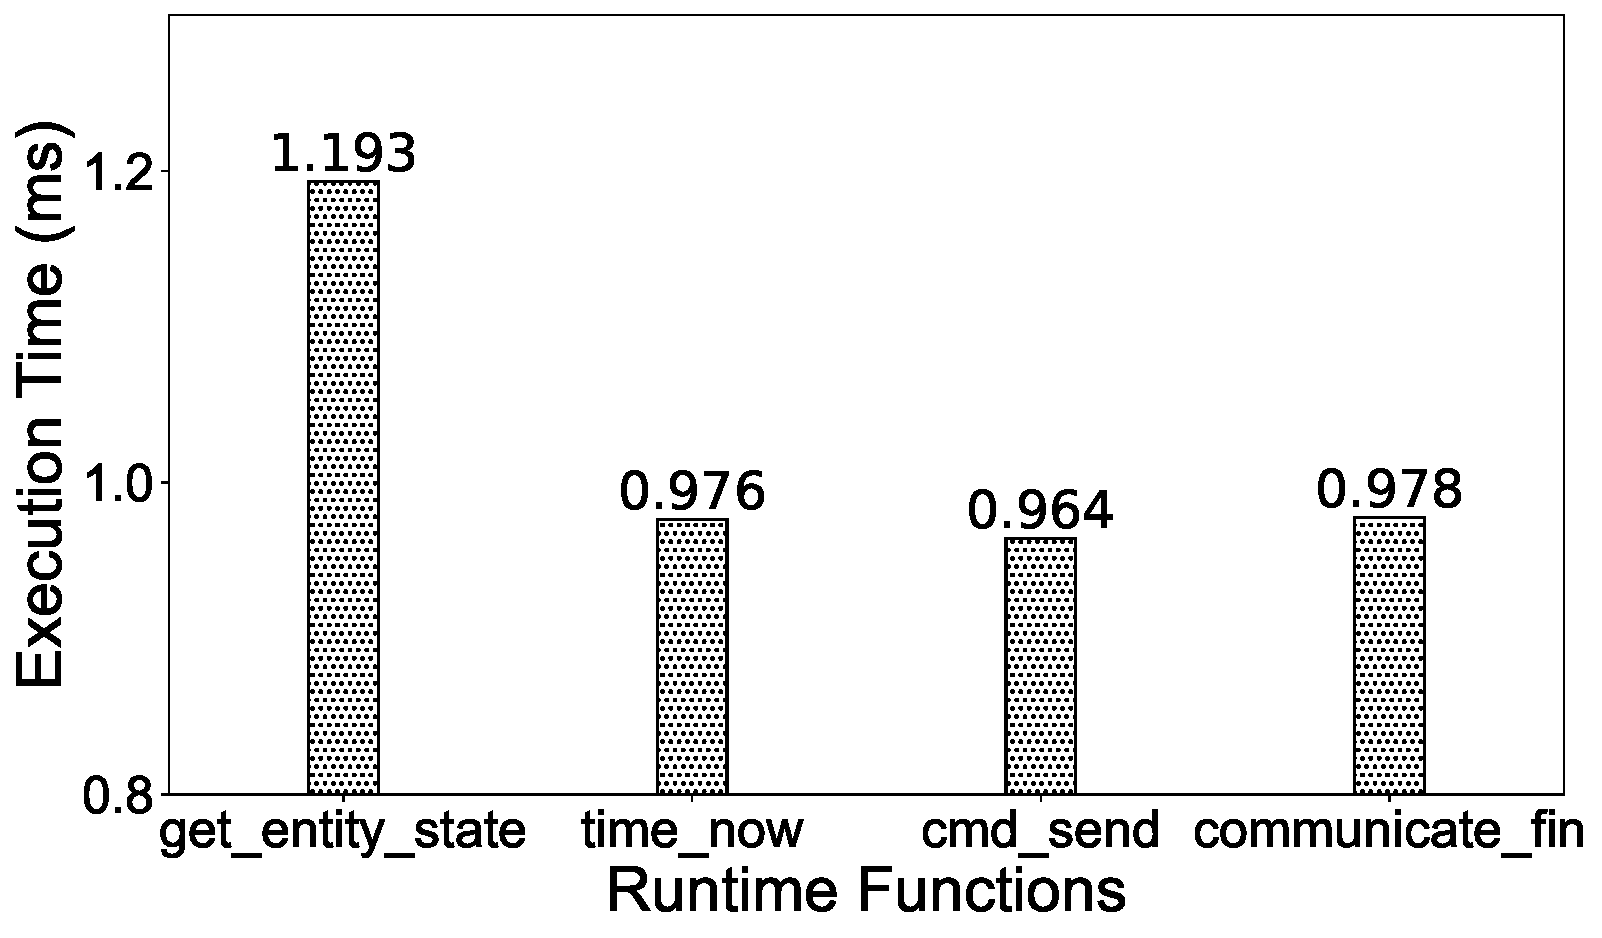
\includegraphics[width=\linewidth]{figure/runtime.pdf}
            \caption{Runtime verification execution time of different functions.}            
            \label{subfig:runtime}
        \end{subfigure}
  \end{minipage}
  \caption{The execution time of different components.}
  \label{fig:performance}
\end{figure*}

We evaluate the execution time of the static and runtime components of the framework.

\textbf{Static analysis.} The static phase constructs TCAE models, builds the RIDG, and extracts the RCDG. Figure~\ref{subfig:static} reports the average execution time on synthetically generated rule sets. Since the analysis checks pairwise interactions among automation rules, the time complexity is $O(n^2)$ for $n$ rules. Nevertheless, the overhead remains acceptable for offline use: the analysis finishes quickly for small and medium-sized rule sets and remains practical even for large rule sets. Because this phase is executed only after rule updates, it does not affect normal runtime operation.

\textbf{Runtime verification.} In the runtime phase, the main overhead comes from state retrieval and timestamp acquisition used by assertion verification. As shown in Fig.~\ref{fig:performance}(b), all runtime functions complete at the millisecond level. Among them, \texttt{get\_entity\_state} incurs the highest latency, while the other functions have similar and slightly lower overhead. Since each assertion verification requires only a small number of such calls, the overall runtime overhead remains low and is suitable for online dynamic monitoring.